\chapter{Implementacion Digital} \chapterlabel{Informe/7-ImplementacionDigital} \label{cap:Implementacion Digital}

\section{Descripción general}

\noindent La implementación digital consiste, básicamente, en realizar la estimación de posición y el control de la planta por medio de un microcontrolador. Se utiliza un kit de desarrollo basado en el microcontrolador STM32F072, que contiene un ADC de 12 bits y 3.3V de referencia, un DAC 12 bits y 3.3V de referencia.

\noindent En la figura \ref{fig:diag-en-bloques-digital} se muestra un diagrama en bloques general de la implementación digital del sistema. Es posible observar que se ingresa al microcontrolador a través de un ADC, con una tensión de referencia ($V_{ref}$) proporcional a la distancia de separación deseada. Esa posición de referencia es comparada con la posición estimada Y(z) y el resultado e(z) es afectado por el compensador digital C(z). Por medio de un DAC, la salida del compensador ingresa al controlador de corriente $G_{iL}(s)$, el cual actúa sobre la planta $G_P(s)$, modificando así la distancia de separación.

\noindent Por medio de un ADC y el sensor de Efecto Hall, se muestrea una tensión proporcional a la corriente que circula por el electroimán. De esta forma, es posible obtener una posición estimada Y(z) al multiplicar esta tensión por la transferencia H(Z).


\begin{figure}[H]
	\centering
	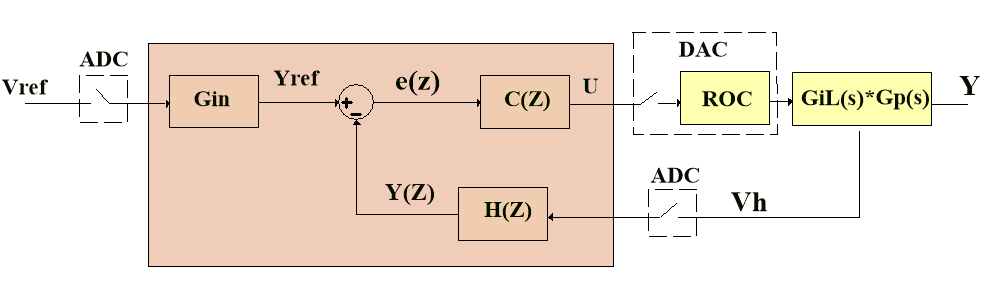
\includegraphics[scale=0.5]{Diagrama-en-bloques-digital.png}
	\caption{Diagrama en bloques de la implementación digital.}
	\label{fig:diag-en-bloques-digital}
\end{figure}

\noindent Abstrayéndose de la matemática que se realiza dentro del micro para la estimación de posición, podemos simplificar el diagrama al que se muestra en la figura \ref{fig:diag-en-bloques-digital-simplif}, en la que:

\begin{equation} 
	G_T(s) = G_P(s) * G_{iL}(s).
\end{equation}

\begin{figure}[H]
	\centering
	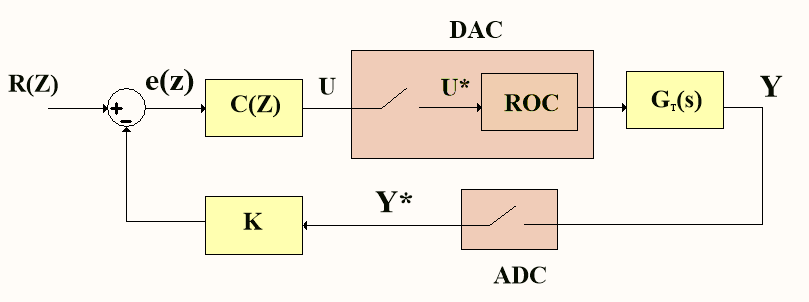
\includegraphics[scale=0.5]{Diagrama-en-bloques-digital-simplificado.png}
	\caption{Diagrama en bloques de la etapa digital simplificado.}
	\label{fig:diag-en-bloques-digital-simplif}
\end{figure}


\section{Determinación de la frecuencia de muestreo}

\noindent Se desea realizar una estimación de la posición del electroimán Y(z)  a partir de las muestras tomadas por el ADC de la tensión de salida del sensor de efecto HALL.

\noindent La forma de onda de la salida del sensor es triangular y presenta una frecuencia variable en función de la inductancia del electroimán, la que, depende de la distancia de separación. Se puede calcular como:

\begin{equation} \label{eq_frecuencia-de-muestreo}
	F_{SW}=\frac{V_{BUS}}{2 * L(y) * \Delta I_H}
\end{equation}

\noindent Dadas las mediciones realizadas sobre el electroimán, se obtuvieron los valores de inductancia al variar la distancia de separación del entrehierro. Al aplicar en la ecuación 5.1 los valores de inductancia obtenidos en la medición (L[mHy]), se calcula la frecuencia de conmutación  $(F_{SW}[Hz])$. Los resultados se muestran en la tabla \ref{frecuencias-calculadas}.


\begin{table}[H]
	\begin{center}
		\begin{tabular}{| c | c | c |}
			\hline
			Y[mm] & L[mHy] & $F_{SW}[Hz]$\\ \hline
			2 & 22.64 & 1060\\ \hline
			3 & 18.8 & 1276\\ \hline
			4.4 & 15.5 & 1548\\ \hline
			5.2 & 14.7 & 1632\\ \hline		
			6.5 & 14.4 & 1666\\ \hline
		\end{tabular}
		\caption{Valores de frecuencia calculados a partir de las mediciones de inductancia realizadas.}
		\label{frecuencias-calculadas}
	\end{center}
\end{table}


\noindent Para la estimación de la posición es necesario medir la pendiente de la onda triangular. Por lo que, para reconstruir su forma de onda es necesario muestrear la señal con cierta cantidad de armónicos para no afectar demasiado la pendiente. Se determinó que la frecuencia de muestreo del ADC debe ser al menos el doble de la frecuencia de la 5º armónica para el caso de la mayor frecuencia. Por lo tanto, se adopta 2.5 veces. Es decir:


\begin{equation} 
	F_S \geq 2.5 * 5 * f_{max} \Rightarrow  F_S \geq 2.5 * 5 * 1666 Hz \Rightarrow F_S \geq 20825 Hz
\end{equation}

\noindent De esta forma, se adopta una frecuencia de muestreo para el ADC de  25 kHz. Por lo tanto, es posible obtener 15 muestras en un período de la triangular para el caso de la frecuencia máxima. Como la señal crece o decrece durante medio ciclo, se pueden tomar 7 muestras para identificar la pendiente. En el caso de que la señal presente la frecuencia mínima, se pueden tomar 23 muestras en un ciclo, lo cual se traduce en 11 muestras para la pendiente de subida o bajada. 


\section{Adquisición y procesamiento de las muestras}

\noindent Considerando el caso de máxima frecuencia, en el que solo se podrán tomar 7 muestras durante el tiempo de crecimiento o decrecimiento, se describe el procedimiento para determinar la posición estimada.


\begin{figure}[H]
	\centering
	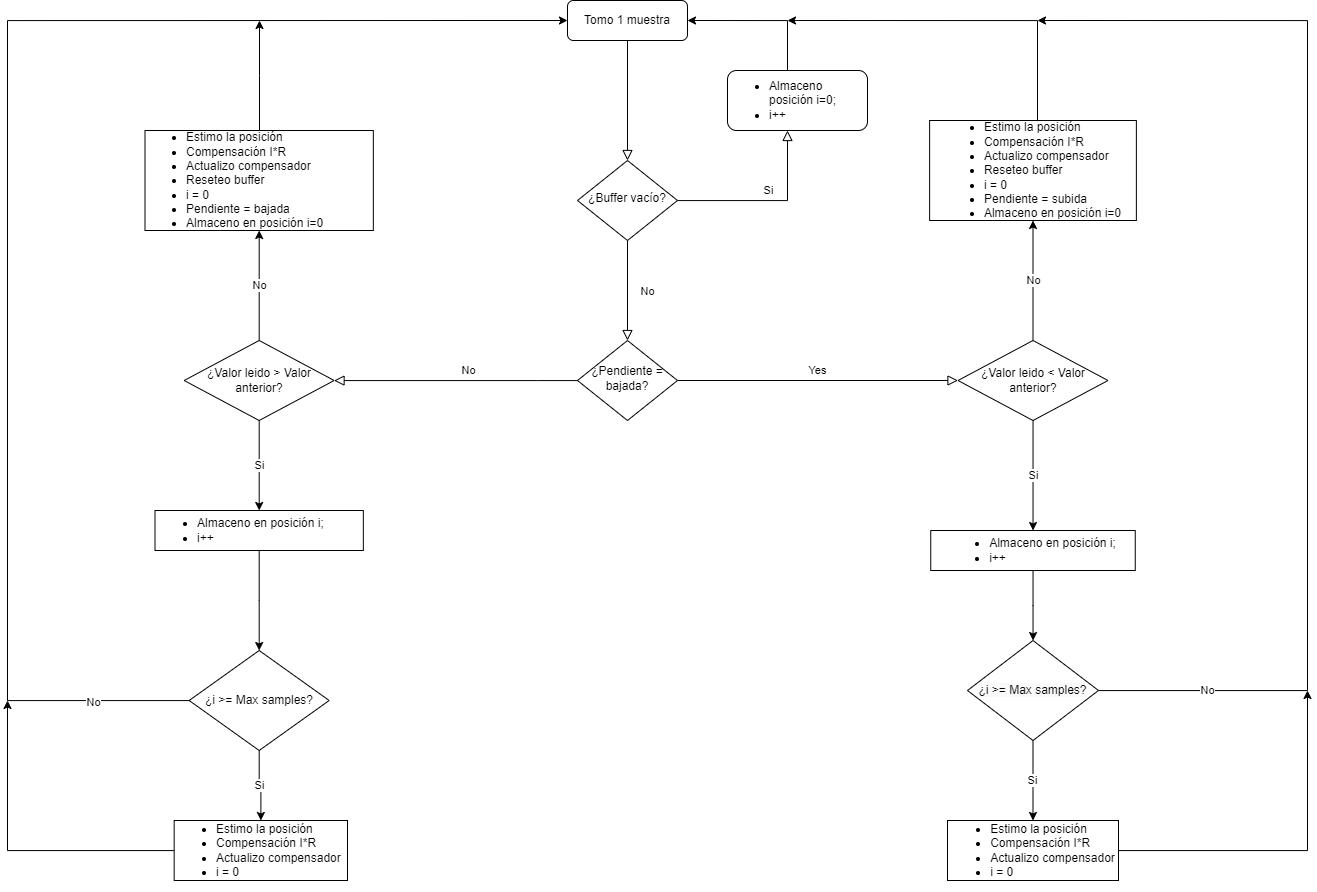
\includegraphics[scale=0.3]{Procesamiento-muestras-adquiridas.png}
	\caption{ Diagrama de flujo del procesamiento de las muestras adquiridas.}
	\label{fig:procesamiento-muestras-adquiridas}
\end{figure}


\noindent Como se observa en el diagrama de flujo de la figura \ref{fig:procesamiento-muestras-adquiridas}, cada muestra de tensión tomada del sensor de efecto hall, se almacena en un buffer de 7 posiciones. Para poder discernir entre pendientes de bajada y de subida, se verifica en cada muestra si el valor leído es mayor o menor al almacenado en la posición anterior. En caso de que sea mayor al anterior, significa que se está muestreando la pendiente positiva de la onda triangular. El hecho de poder discernir entre pendientes positivas y negativas, permite aplicar la compensación I*R al igual que se realiza en el estimador analógico. 

\noindent Cada vez que el buffer se complete, se realiza el cálculo de la derivada con el valor máximo y mínimo almacenado. Con este resultado, se hace la estimación de la posición y se actualiza la entrada al compensador digital.

\noindent En caso de haber completado las 7 posiciones del buffer y la pendiente persiste con el mismo signo, el buffer comienza a llenarse nuevamente desde la posición inicial, sobreescribiendo los valores de mayor vejez. Por lo tanto, pueden ocurrir dos situaciones. La primera es que se detecte un cambio de pendiente antes de completar nuevamente el buffer, con lo cual se calcula la derivada con los valores extremos almacenados sin importar su vejez y se actualiza la entrada al compensador. La segunda, es que se vuelva a completar el buffer, en cuyo caso también se hace la actualización. La diferencia entre estas dos situaciones es el tiempo transcurrido. En este último, se hace cada 7 períodos de muestreo mientras que en el primero se realiza “N” períodos de muestreo luego de la última actualización, donde “N” representa la cantidad de muestras que se almacenaron en el buffer incompleto.

\noindent Luego de cada actualización, el proceso vuelve a iniciar con el buffer vacío.

\noindent Utilizando este método de estimación, puede ocurrir que se obtenga una nueva estimación en 7 periodos de muestreo del ADC, o incluso en menos. Por lo tanto se podría decir que se tiene un estimador de posición con frecuencia de actualización variable. Esto es importante al momento de diseñar un compensador digital para el sistema. Para hacerlo, se debe considerar el caso en que la frecuencia de actualización es la menor, por lo tanto podríamos decir que el compensador digital se debe diseñar con una frecuencia de muestreo de 25/7 KHz = 3.5 KHz.

\section{Estimación digital de la posición}

\noindent De las mediciones realizadas se llegó a la expresión que relaciona la distancia de separación con la pendiente de la corriente en el electroimán:

\begin{equation} 
	|\frac{di_L}{dt}[A/s]| = 194690 * Y[m] + 676 [A/s]
\end{equation}

\noindent Por lo tanto, la posición en metros puede despejarse como:

\begin{equation} 
	Y = 5.136*10^{-6}*|\frac{di_L}{dt}|- 3.472*10^{-3} [m]
\end{equation}

\noindent Es importante notar que la resistencia interna (R) del electroimán genera una caída de tensión cuando circula corriente. Esta caída provoca que la tensión efectiva aplicada sobre la inductancia sea distinta para el semiciclo de subida que el de bajada, generando que la onda triangular tenga diferentes pendientes (en valor absoluto) para cada caso. Esta se representa como $(\frac{di_L}{dt})_{Real}$ y es la que se mide al utilizar el ADC.

\noindent Es decir:

\begin{equation} 
	(\frac{di_L}{dt})_{Real}=(\frac{di_L}{dt})_{Teorica}-\frac{R*I_L}{L(y)}
\end{equation}

\noindent Aproximando la derivada real como la resta entre la muestra en un instante menos el anterior sobre el período de muestreo y compensando el error que introduce la resistencia interna, se obtiene:

\begin{equation} 
	Y = 5.136*10^{-6}* |\frac{I_L[n]-I_L[n-1]}{T_S}+\frac{R*i_L}{L(y)}| - 3.472*10^{-3} [m]
\end{equation}


\noindent Considerando a $V_h$ como la tensión entregada por el sensor de efecto hall, proporcional a la corriente que circula por el electroimán multiplicada por una ganancia $K_h$ de 53.3mV/A, donde  ($\hat{V_h}$)  corresponde a la componente alterna de tensión y ($\bar{V_h}$) la continua, resulta:


\begin{equation} 
	V_h[n] = \bar{V_h}[n] + \hat{V_h}[n] = K_h * (\bar{I_L}[n] + \hat{I_L}[n])
\end{equation}

\noindent Para la estimación de la posición se utiliza el término de alterna mientras que para compensar el error introducido por la resistencia interna del electroimán se utiliza el de continua. Por lo tanto, se obtiene:

\begin{equation}
	Y = 5.136*10^{-6}*|\frac{\hat{V_h}[n]-\hat{V_h}[n-1]}{K_h*T_S} + \frac{R*\bar{V_h}[n]}{K_h*L(y)[n-1]}|-3.472*10^{-3}[m]
\end{equation}

\noindent El valor de corriente $\bar{V_h}[n]$ se obtiene de sensar el valor medio de tensión entregado por el sensor de efecto Hall mediante otro canal del ADC.

\noindent Por otro lado, el valor de L(y)[n-1] se obtiene de aplicar el valor anterior estimado de posición en la ecuación \ref{eq_inductancia}. El cálculo de esta expresión se obtiene a partir de la linealización de la inductancia en función de las mediciones realizadas sobre el electroimán.

\begin{equation} \label{eq_inductancia}
	L(y)[n-1] = -2.56*Y[n-1]+0.0271 Hy
\end{equation}

\noindent Por lo tanto la ecuación correspondiente en el tiempo discreto:

\colorbox{yellow}{-------------------------------acomodar tamaño de ecuaciones-------------}
\begin{equation}
	Y = 5.136*10^{-6}*|\frac{\hat{V_h}[n]-\hat{V_h}[n-1]}{K_h*T_S} + \frac{R*\bar{V_h}[n]}{K_h*(2.56*Y[n-1]+0.0271)}|-3.472*10^{-3}[m]
\end{equation}

\begin{equation}
	Y = 96.3*10^{-6}*|\frac{\hat{V_h}[n]-\hat{V_h}[n-1]}{T_S} + \frac{R*\bar{V_h}[n]}{(2.56*Y[n-1]+0.0271)}|-3.472*10^{-3}[m]
\end{equation}


\noindent Donde n representa el número de muestras. Es decir, $V_h[n]$ se refiere a la muestra más reciente en el buffer y $V_h[n-1]$ a la más vieja.

\noindent Es importante notar que los coeficientes deben calcularse antes de actualizar el compensador en función de la cantidad de períodos de muestreo transcurridos desde la última actualización. Estos deben calcularse en ese momento puesto que el compensador digital presenta una frecuencia de actualización variable y los coeficientes del estimador dependen de ella.

\noindent Por otro lado, el bloque K mostrado en la Figura \ref{fig:diag-en-bloques-digital-simplif} resulta en una transferencia unitaria.

\section{Resolución en posición}

\noindent Una variación de posición ($\Delta Y$) produce un cambio de inductancia ($\Delta L[y]$) que se traduce en un cambio de frecuencia ($\Delta f$). Para poder detectar el mínimo cambio de posición en un período de muestreo se debe tener una resolución tal que permita discernir ese cambio de frecuencia.

\noindent A partir de los valores de inductancia  obtenidos con las mediciones, es posible realizar una aproximación lineal como se muestra en la ecuación \ref{eq_inductancia-linealizada}.

\begin{equation} \label{eq_inductancia-linealizada}
	L[Hy] = -2.56 * Y[m] + 0.0271 Hy
\end{equation}

\noindent Aplicando la expresión linealizada de la inductancia y la ecuación \ref{eq_frecuencia-de-muestreo} es posible obtener el valor de frecuencia para una separación de Y=2.1mm. Este resulta de $f_{SW}[2.1mm] = 1104.8 Hz$. De esta forma, conociendo el valor de frecuencia para 2 mm, el cual es de $f_{SW}[2mm] = 1060 Hz$, es posible obtener la variación de frecuencia para un Y mínimo de 0.1mm. Este valor puede obtenerse como:

\begin{equation} 
	\Delta F_{SW}(Teorico) = f_{SW}[2.1mm] - f_{SW}[2mm] = 44.8 Hz
\end{equation}

\noindent Las pendientes para el peor caso se da con la menor variación de tensión entre muestras. Es decir, para el caso de frecuencia mínima. En la ecuación \ref{eq_pendiente} se muestra el cálculo de la pendiente de la onda triangular en función de la frecuencia de conmutación.

\begin{equation} \label{eq_pendiente}
	P(f_{SW}) = \frac{\Delta V}{T_{SW}/2} = 2*K_H*\Delta i_L*f_{SW} = 2 * 0.0533 * 0.5 * f_{SW}
\end{equation}

\noindent A partir de la ecuación \ref{eq_pendiente} es posible obtener el valor de la pendiente para la frecuencia mínima de conmutación y la de su incremento correspondiente a una variación en la posición de 0.1mm. Esta situación se representa en la figura \ref{fig:variacion-de-pendiente}.

\begin{equation} 
	\begin{aligned}
		P(f_{SW_{min}}) &= 56.49 [V/s] \\
		P(f_{SW_{min}} + \Delta f_{SW}) &= 58.89 [V/s] \\
	\end{aligned}
\end{equation}


\begin{figure}[H]
	\centering
	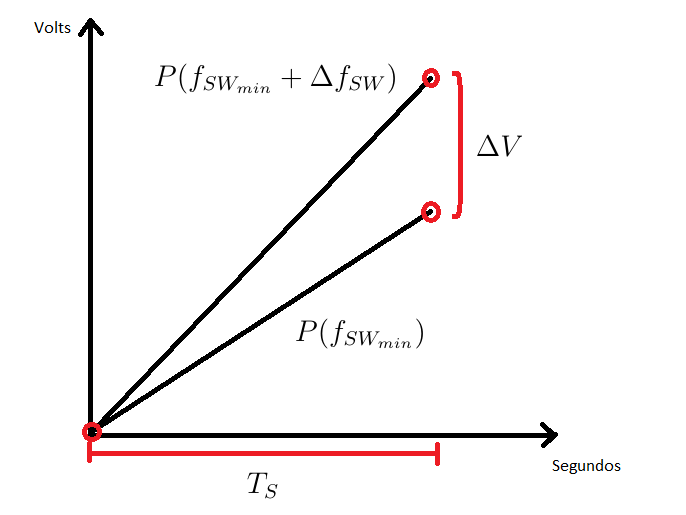
\includegraphics[scale=0.3]{Variacion-de-pendientes.png}
	\caption{Variación de pendiente ante mínimo cambio de posición.}
	\label{fig:variacion-de-pendiente}
\end{figure}

\noindent Por lo tanto, para poder diferenciar las pendientes, la resolución del ADC debe ser menor o igual a $\Delta V$.

\begin{equation} 
	\begin{aligned}
		V1 &= P(f_{SW_{min}} + \Delta f_{SW})* T_S \\
		V2 &= P(f_{SW_{min}})* T_S \\		 
	\end{aligned}
\end{equation}

\noindent Al considerar $T_s = 125 kHz$:

\begin{equation} 
	\Delta V_{ADC} = T_S * [P(f_{SW_{min}} + \Delta f_{SW}) - P(f_{SW_{min}})] = 96 \mu V
\end{equation}



\noindent Este resultado indica que al usar un ADC de 12 bits, se necesitaría una tensión de referencia $V_{ref} = 0.393216 V$. Sin embargo, este valor resulta demasiado bajo y no sirve si se quiere medir la salida del sensor de efecto Hall de manera directa. Por lo tanto, se decide diseñar un circuito que permita realizar la estimación manteniendo la tensión de referencia en 3.3V

\noindent La corriente que circula por el electroimán presenta una componente de continua y otra de alterna. La primera excursiona entre 0A y 30A mientras que la segunda varía entre $\pm 250 mA$ en torno al valor medio, con forma de onda triangular. Es posible hacer una adquisición separada de ambas componentes con el ADC para que luego sean procesadas. La señal que ingresa al circuito corresponde a la tensión de salida del sensor de efecto Hall sin el set point de 2.5V.

\noindent Si se tiene en cuenta la ganancia del sensor de efecto Hall, a su salida se obtiene una señal cuyo valor medio varía entre 0 y 1.6 V, y un valor de alterna de $26.7 mV_{pp}$.

\noindent Debido a que el ADC permite una excursión entre 0V y 3.3V, la máxima ganancia posible es de 60 veces para la señal de alterna. Por otro lado, para medir con la resolución en posición deseada de 0.1 mm se debe amplificar la señal triangular 9 veces como mínimo.

\noindent Por lo tanto, se adopta una ganancia de 50, obteniendo así una excursión máxima de 3.17V (0.67V sobre el set-point).

\noindent Las características del circuito son:

\begin{itemize}
	\item Ganancia: 50
	\item Set-point de 2.5V 
	\item Frecuencia de corte inferior: 100 Hz
	\item Frecuencia de corte superior: 12,5 kHz
\end{itemize}

\noindent Teniendo en cuenta la ganancia elegida,  la pendiente de la onda triangular resulta:

\begin{equation} 
	P(F_{SW}) = 50 * [0.0533 * 0.5 * (F_{SW}*2)][\frac{V}{s}]
\end{equation}

\noindent Reemplazando para el incremento de frecuencia se obtiene los valores 

\begin{equation} 
	\begin{aligned}
		P(f_{SW_{min}} &= 2824.9 \ [\frac{V}{s}]\\
		P(f_{SW_{min}} + \Delta f_{SW}) &= 2944.29 \ [\frac{V}{s}]\\		 
	\end{aligned}
\end{equation}

\noindent Entonces, 

\colorbox{yellow}{--------------------Ver largo de ecuación--------------------}

\begin{equation} 
	\Delta V_{ADC} = T_S * [P(f_{SW_{min}} + \Delta f_{SW}) - P(f_{SW_{min}})] = 0.1177 V - 0.1129 V = 4.7mV
\end{equation}


\noindent Por lo tanto, como la resolución del ADC es de 0.8mV, resulta suficiente para identificar el mínimo cambio de pendiente.


\section{Acondicionamiento de señales para el ADC}

\subsection{Referencia de posición}

\noindent Para indicar al microcontrolador la distancia de separación deseada se utiliza una señal continua como referencia que se ajusta desde un potenciómetro ubicado en el PCB (al igual que para el compensador analógico) e ingresa al circuito mostrado en la figura \ref{fig:circuito-ref-posicion}. Debido a que entrega una tensión entre 3.96V y 4.69V, se implementa un circuito de acondicionamiento para esta señal.

\noindent A la señal de entrada se le resta el setpoint de 2.5 V, para lograr señales que van desde 1.42V a 2.2V. Luego dentro del microcontrolador se debe mapear el valor leído por el ADC con la posición deseada usando la ganancia del estimador analógico según la fórmula:

\begin{equation} 
	Y_{ref}\ =\frac{Vpo{s_{ref}}_{ADC}\ +\ 2.5V}{259.6}\ [m]
\end{equation}

\noindent Además se implementa un filtro anti-aliasing con frecuencia de corte en 9.9 kHz.

\begin{figure}[H]
	\centering
	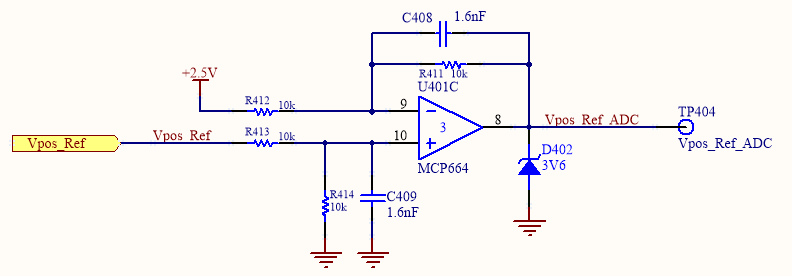
\includegraphics[scale=0.5]{Circuito-ref-posicion.png}
	\caption{Circuito acondicionador para componente alterna de corriente del electroimán.}
	\label{fig:circuito-ref-posicion}
\end{figure}

\subsection{Componente  continua de corriente del electroimán}

\noindent Para obtener solamente la componente alterna de la corriente, se implementa un circuito con característica pasa-banda que se muestra en la figura \ref{fig:componente-corriente-alterna}. La frecuencia de corte inferior  es de 100Hz, con el objetivo de eliminar el valor medio de señal. Por otro lado, la superior es de 12 KHz, que actúa como filtro anti-aliasing. Luego la salida es amplificada con una ganancia de 50 veces (con el objetivo de mejorar la medición de la pendiente por el ADC) y montada sobre un set-point de 2.5V.

\begin{figure}[H]
	\centering
	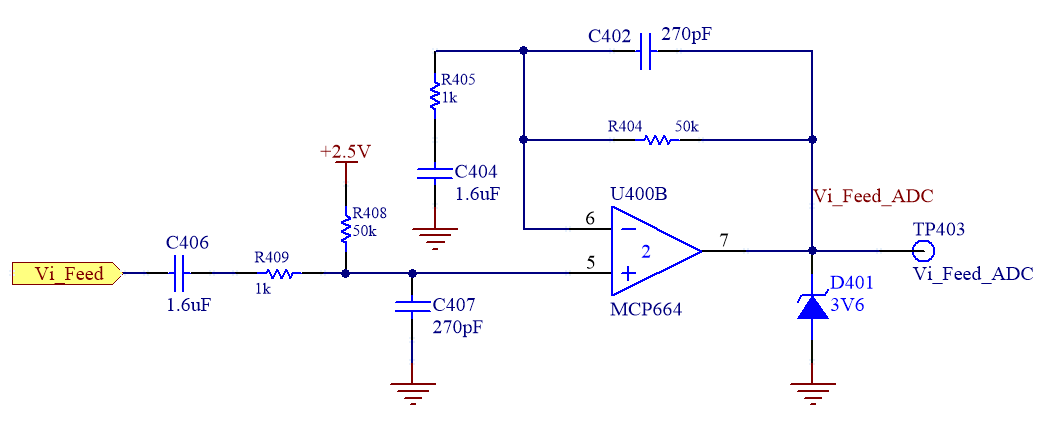
\includegraphics[scale=0.5]{Componente-corriente-alterna.png}
	\caption{ Circuito acondicionador para componente alterna de corriente del electroimán.
	}
	\label{fig:componente-corriente-alterna}
\end{figure}

\subsection{Componente  continua de corriente del electroimán}

\noindent Para obtener la componente de contínua se utiliza un filtro pasa-bajos con frecuencia de corte en 106 Hz. Se eligió esta frecuencia para que se ubique por lo menos una década por debajo de la frecuencia fundamental de la onda triangular. La implementación circuital puede observarse en la figura \ref{fig:componente-corriente-continua}


\begin{figure}[H]
	\centering
	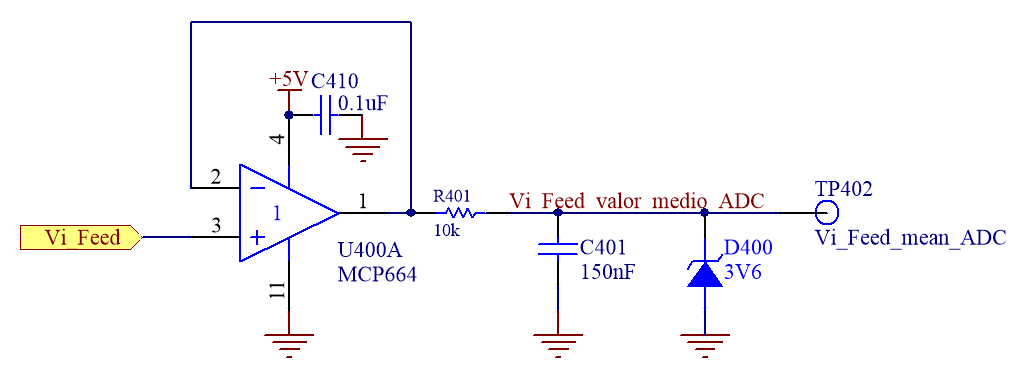
\includegraphics[scale=0.5]{Componente-corriente-continua.png}
	\caption{Circuito acondicionador para componente continua de corriente del electroimán.
	}
	\label{fig:componente-corriente-continua}
\end{figure}

\section{Acondicionamiento de señales para el DAC}

\noindent Para convertir los valores digitales de la estimación de posición y de la compensación al dominio analógico, se utilizan los DAC del microcontrolador. La tensión entregada es afectada por una circuitería de filtrado, ganancia y protección como se muestra en las figuras \ref{fig:DAC-compensador} y \ref{fig:DAC-estimador}. Debido a que el DAC se actualiza con una frecuencia mínima de 3.5 KHz, se utilizan filtros con frecuencia de corte en 1.75KHz.

\noindent Por otro lado, como el controlador de corriente funciona con tensiones de hasta 5 V en su entrada y el compensador fue diseñado teniendo en cuenta este nivel de tensión, se agrega una ganancia por firmware de 0,66, mapeando así los 5 V a 3,3 V, que es la máxima tensión entregada por el DAC. Luego, para compensar esta ganancia y no afectar a la transferencia de la planta, se la afecta por un factor de de $\frac{5V}{3.3V}$ por medio del circuito de acondicionamiento.

\noindent De esta forma, se logra convertir correctamente la señal digital en analógica.


\begin{figure}[H]
	\centering
	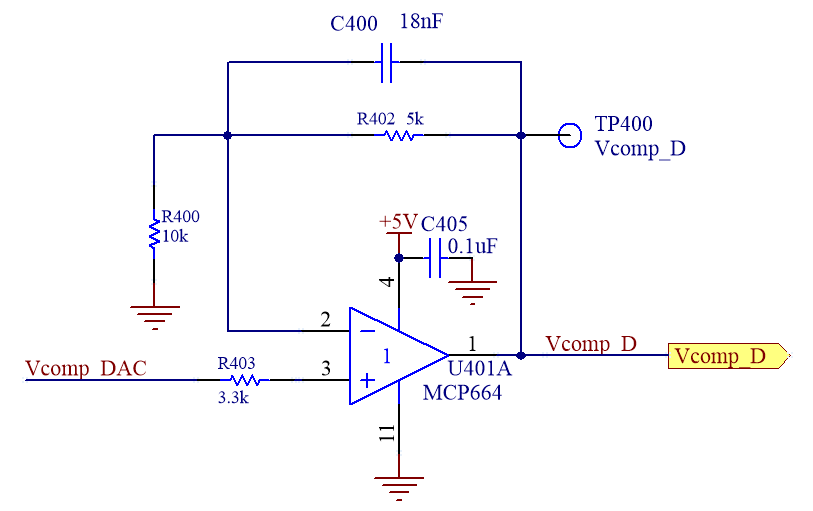
\includegraphics[scale=0.5]{DAC-compensador.png}
	\caption{Circuito acondicionador para la salida del DAC correspondiente al compensador.}
	\label{fig:DAC-compensador}
\end{figure}

\begin{figure}[H]
	\centering
	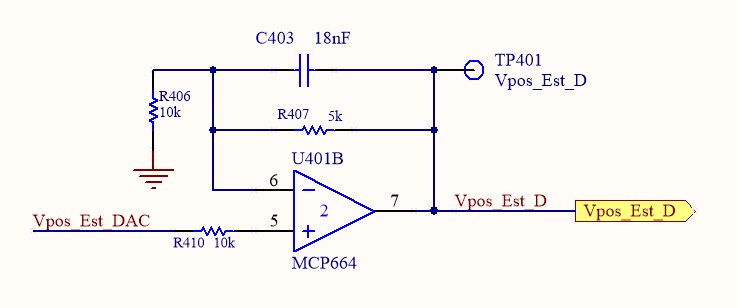
\includegraphics[scale=0.5]{DAC-estimador.png}
	\caption{Circuito acondicionador para la salida del DAC correspondiente al estimador digital.}
	\label{fig:DAC-estimador}
\end{figure}

\section{Transferencias de la planta y del controlador de corriente}

\noindent Para el an\'{a}lisis del compensador digital, se parte de las transferencias de la planta $G_P(s)$ y del controlador de corriente $G_{iL}(s)\ $ en dominio anal\'{o}gico para una masa de 30 Kg.

\begin{equation} 
	\begin{aligned}
	G_T(s)[30Kg]&=G_P(s)*G_{iL}(s)\\
	G_T(s)[30Kg]&=\frac{245*{10}^{-6}}{{1-(\frac{s}{70})}^2}*\frac{6}{\frac{S}{12.17\ }+1\ }\\
	G_T(s)[30Kg]&=\frac{-87.7}{\ (s-70)\ (s+70)\ (s+12.17)}\\
	\end{aligned}
\end{equation}

\noindent Al aplicar la transformada z por invarianza al impulso, considerando una $f_s=3.5\ KHz$, se obtiene:

\begin{equation} 
	G_T(Z)[m=30\ Kg]\ \ =\frac{-3.4*10^{-10}(z+3.7)(z+0.3)}{\ (z-0.9965)\ (z+0.9802)\ (z+0.2677)}
\end{equation}

\noindent Luego, usando la transformada bilineal para volver al dominio anal\'{o}gico:
\\
 \colorbox{yellow}{----------------ver largo de ecuacion------}
\begin{equation} 
	G_T(w)[m=30\ Kg]\ \ =\frac{-8.5*10^{-11}(w-1.21*10^4)(w-7000)(w+1.21*10^4)}{\ (w-70)\ (w+70)\ (w+12.17)}
\end{equation}


\noindent Con las expresiones en [W], es posible dise\~{n}ar un controlador de manera anal\'{o}gica, para luego transformarlo al dominio digital.


\section{Diseño de Compensador}

\subsection{Análisis de estabilidad con masa de 30 Kg}

\noindent Considerando que la ganancia de avance est\'{a} formada por la planta y el controlador de corriente y que el lazo de realimentaci\'{o}n es unitario, se procede a analizar la respuesta en frecuencia de ${GH}_T$ para una masa de 30 Kg y a dise\~{n}ar un compensador adecuado. Luego, se verifica la estabilidad para una masa de 1 Kg, que corresponde a la m\'{i}nima con la que trabaja el sistema.
 
\begin{equation} \label{eq_TLC-lazo-abierto} 
	G_T(w)*H(w)=\frac{-8.5*10^{-11}(w-1.21*10^4)(w-7000)(w+1.21*10^4)}{\ (w-70)\ (w+70)\ (w+12.17)} 
\end{equation} 


\noindent Con la transferencia de la ecuación \ref{eq_TLC-lazo-abierto} se  grafica el diagrama de Bode y el diagrama de Nyquist que se muestran en las figuras \ref{fig:bode-lazo-abierto-digital} y \ref{fig:nyquist-lazo-abierto-digital} respectivamente.

\begin{figure}[H]
	\centering
	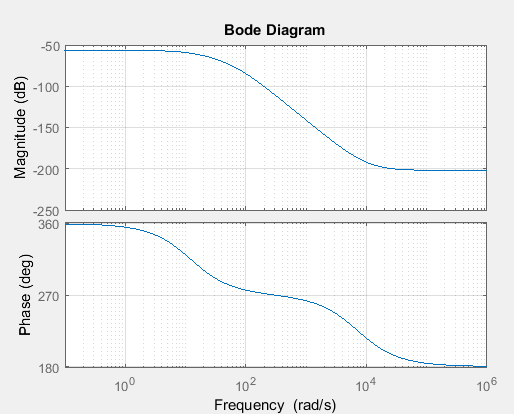
\includegraphics[scale=0.6]{Bode-lazo-abierto-digital.png}
	\caption{Diagrama de Bode de lazo abierto GHT con M=30 Kg.}
	\label{fig:bode-lazo-abierto-digital}
\end{figure}

\begin{figure}[H]
	\centering
	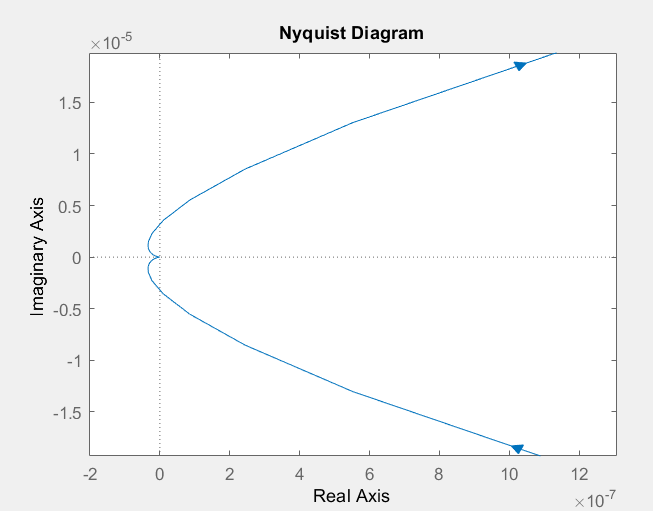
\includegraphics[scale=0.8]{Nyquist-lazo-abierto-digital.png}
	\caption{Diagrama de Nyquist de GHT con M=30 Kg.}
	\label{fig:nyquist-lazo-abierto-digital}
\end{figure}

\noindent Considerando que ${GH}_T$ tiene un polo en el semiplano derecho, a partir del Nyquist se puede determinar:

\noindent Zona 1: Z=N+P=0+1=1 $\mathrm{\to}$ Inestable 

\noindent Zona 2: Z=N+P=1+1=2 $\mathrm{\to}$ Inestable

\noindent De esta forma, no es posible que el sistema sea estable. Para lograrlo se realimentar\'{a} positivamente y se generar\'{a} una zona en el diagrama de Nyquist donde N=-1. Para ello es necesario aumentar la fase para que pueda superar el valor de 0$\mathrm{{}^\circ}$.  Para que esto se cumpla, el diagrama de Nyquist deber\'{i}a tener una forma como la  mostrada en la figura \ref{fig:nyquist-deseado-digital}.

\begin{figure}[H]
	\centering
	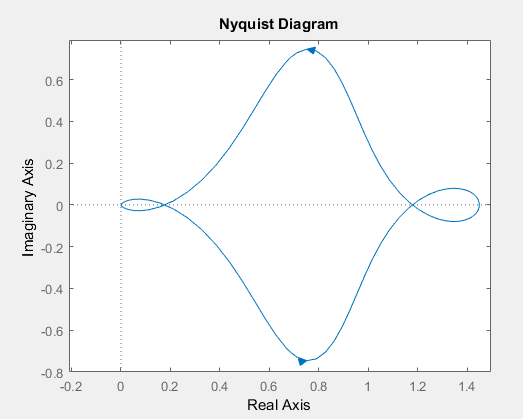
\includegraphics[scale=0.7]{Nyquist-deseado-digital.png}
	\caption{Forma del diagrama de Nyquist deseado.}
	\label{fig:nyquist-deseado-digital}
\end{figure}

\noindent Para poder lograr el aumento de fase mencionado se utiliza una red de adelanto de fase. Se debe tener en cuenta que el m\'{o}dulo de la transferencia de lazo abierto en el primer cruce de la fase por 0$\mathrm{{}^\circ}$ debe ser mayor a 0 dB y, en el segundo cruce, menor. De esta forma, al observar la figura \ref{fig:bode-lazo-abierto-digital} se decide adelantar la fase 100º en aproximadamente 200 rad/s. Esto se logra usando dos redes de adelanto de fase de 65$\mathrm{{}^\circ}$ cada una.

\noindent Ecuaciones de dise\~{n}o:

\begin{equation}
	\begin{aligned}
		W_0 &=200\ r/s\\
		{\varphi }_{max} &=65\textrm{º}\\
		\alpha &=\frac{1+sen{\varphi }_{max}}{1-sen{\varphi }_{max}}=20.346491\\
		W_c &=\frac{W_0}{\sqrt{\alpha }}=\ 44.3\ r/s\\
		W_p &=\sqrt{\alpha }*W_0=902.1\ r/s\\
	\end{aligned}
\end{equation} 
\noindent Finalmente se llega a la transferencia del controlador:

 \begin{equation}  
 	G_c(s)=K*{[20.346*\frac{(s+44.3)}{(s+902.1)}]}^2
 \end{equation} 
 


\noindent En la figura \ref{fig:bode-compensado-para-k-1} se muestra el diagrama de bode de ${GH}_T*G_C$ con $K=1$. Se puede observar que la ganancia $K$ puede adoptar valores desde 64 dB hasta 89.5 dB. Considerando que el sistema debe soportar una masa variable entre 1 kg y 30 kg, y que la ganancia de la transferencia de la planta para 1 kg es de 5.5 veces (14 dB) mayor que para 30 kg, se puede adoptar una ganancia del compensador que mantenga la estabilidad para estos dos casos. Es decir, la ganancia m\'{i}nima es de 64 dB y la m\'{a}xima es de 89.5 dB - 14 dB = 75.5 dB. Por lo tanto, se elige que el cruce por cero de la ganancia se encuentre ahora en 88 rad/s, lo que significa que $K=68.4dB\ \equiv \ 2630\ veces$.


\begin{figure}[H]
	\centering
	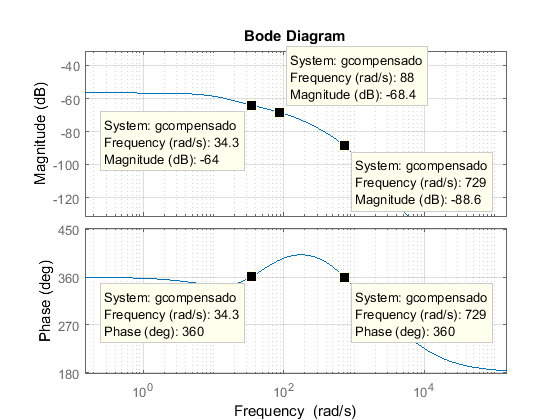
\includegraphics[scale=0.7]{Bode-compensado-para-k-1.png}
	\caption{Diagrama de Bode de GHT*GC para K=1 y M=30 Kg.}
	\label{fig:bode-compensado-para-k-1}
\end{figure}


\noindent En la figura \ref{fig:bode-compensado-para-k-2630} se muestra el diagrama de Bode considerando la ganancia del compensador. En ella se puede observar que se  cumple con el criterio de estabilidad, puesto que en el primer cruce por 0º, la magnitud es mayor a 0 dB y en el segundo cruce, menor. Adem\'{a}s, en la figura \ref{fig:nyquist-para-k-2630} se puede ver que la forma del diagrama de Nyquist es como la deseada.

\begin{figure}[H]
	\centering
	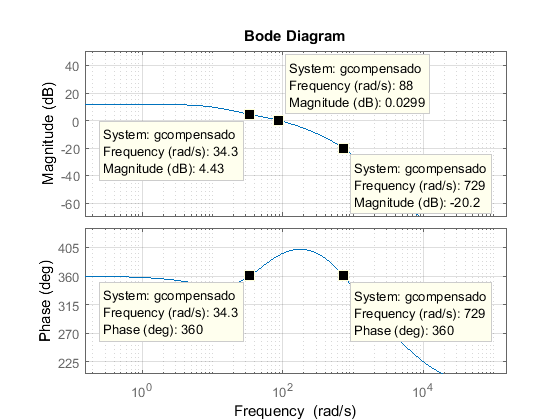
\includegraphics[scale=0.7]{Bode-compensado-para-k-2630.png}
	\caption{Diagrama de Bode de GHT*GC para K=2630 y M=30 Kg.}
	\label{fig:bode-compensado-para-k-2630}
\end{figure}

\begin{figure}[H]
	\centering
	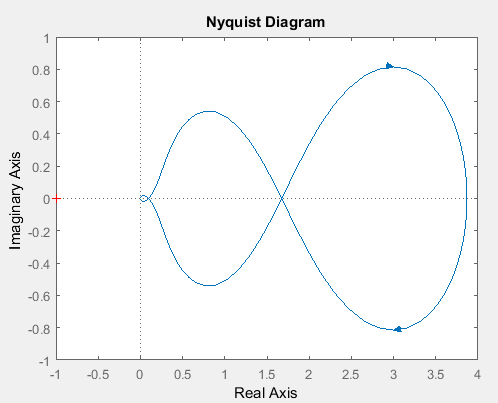
\includegraphics[scale=0.7]{Nyquist-para-k-2630.png}
	\caption{Diagrama de Nyquist de GHT*GC para K=2630 y M=30 Kg.}
	\label{fig:nyquist-para-k-2630}
\end{figure}

\noindent En la figura \ref{fig:respuesta-al-escalon-para-M-30} se puede observar la respuesta al escal\'{o}n del sistema con masa de 30 Kg.


\begin{figure}[H]
	\centering
	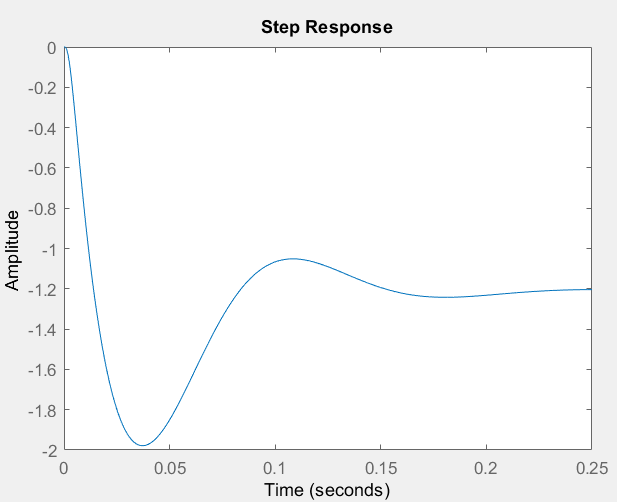
\includegraphics[scale=0.9]{Respuesta-al-escalon-para-M-30.png}
	\caption{Respuesta al escalón para M=30 Kg.}
	\label{fig:respuesta-al-escalon-para-M-30}
\end{figure}

\subsection{Análisis de estabilidad con masa de 1 Kg}

\noindent En esta secci\'{o}n se verifica la estabilidad del sistema  para el caso en que la masa sea de 1 Kg, utilizando el compensador dise\~{n}ado para el caso de masa m\'{a}xima. Para ello, se analizan los diagramas de Bode y Nyquist mostrados en las figuras \ref{fig:bode-para-M-1Kg} y \ref{fig:nyquist-para-M-1Kg}. Adem\'{a}s, en la figura \ref{fig:respuesta-al-escalon-para-M-1Kg} puede observarse la respuesta al escal\'{o}n. A partir de ellos, es posible verificar que efectivamente el sistema resulta estable para todo el rango de masas en el que opera el sistema. 


\begin{figure}[H]
	\centering
	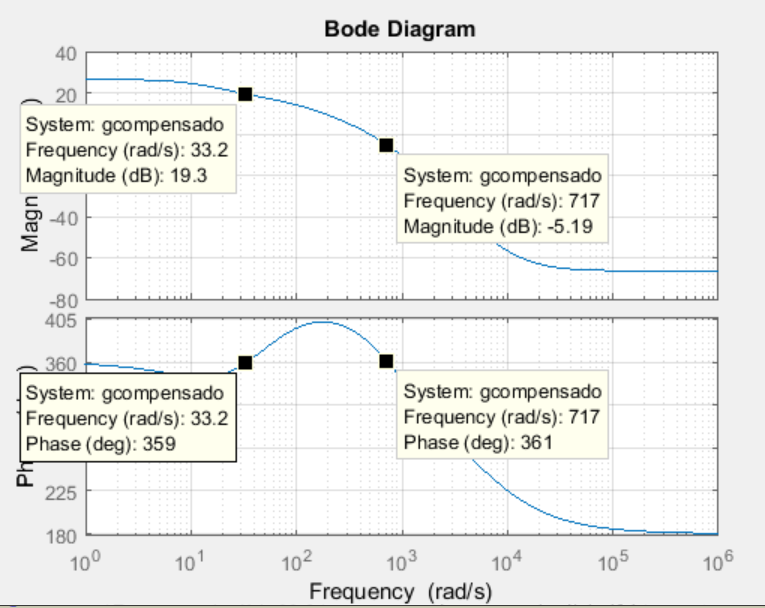
\includegraphics[scale=0.4]{Bode-para-M-1Kg.png}
	\caption{Diagrama de Bode de $GH_T*G_C$ para M=1 Kg.}
	\label{fig:bode-para-M-1Kg}
\end{figure}

\begin{figure}[H]
	\centering
	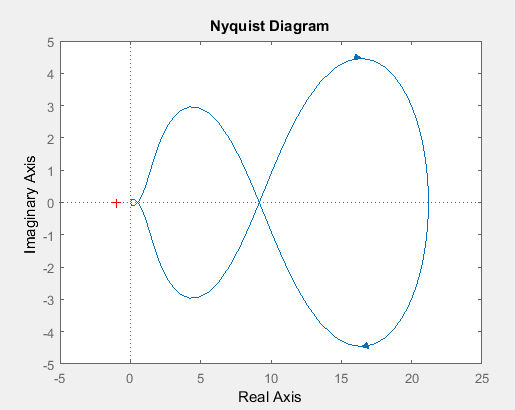
\includegraphics[scale=0.6]{Nyquist-para-M-1Kg.png}
	\caption{Diagrama de Nyquist de $GH_T*GC$ para M=1 Kg.}
	\label{fig:nyquist-para-M-1Kg}
\end{figure}

\begin{figure}[H]
	\centering
	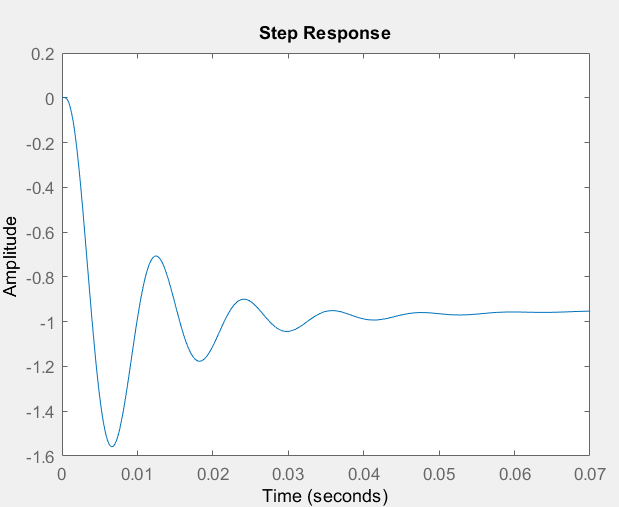
\includegraphics[scale=0.8]{Respuesta-al-escalon-para-M-1Kg.png}
	\caption{Respuesta al escalón para M=1 Kg.}
	\label{fig:respuesta-al-escalon-para-M-1Kg}
\end{figure}

\section{Diseño de lazo de realimentación externo}

\noindent Se plantea un lazo de realimentaci\'{o}n externo como se muestra en la  figura \ref{fig:diagrama-del-sistema-completo}.

\begin{figure}[H]
	\centering
	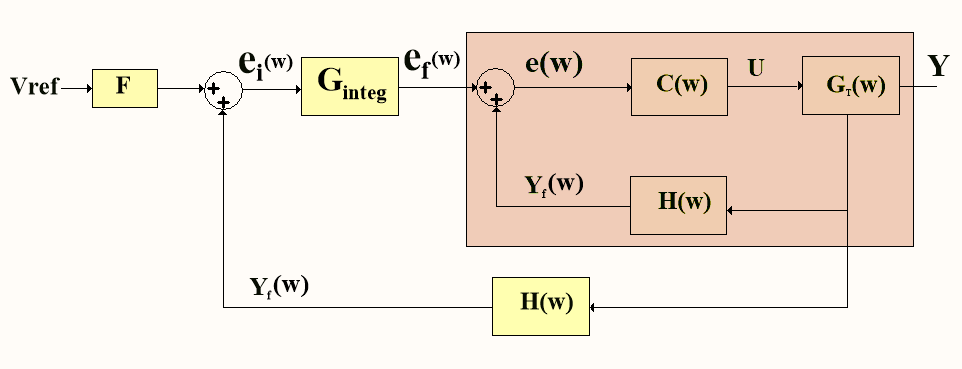
\includegraphics[scale=0.4]{Diagrama-del-sistema-completo.png}
	\caption{Diagrama del sistema completo.}
	\label{fig:diagrama-del-sistema-completo}
\end{figure}









